\documentclass{article}
\usepackage{amsmath}
\usepackage{amssymb}
\usepackage{graphicx}
\usepackage{hyperref}
\usepackage[version=4]{mhchem}

\title{Problem 5}
\date{}

\begin{document}
\maketitle

\section*{Problem}
(2003 AMC 10B Problem 20). In rectangle \(A B C D, A B=5\) and \(B C=\) 3. Points \(F\) and \(G\) are on \(C D\) so that \(D F=1\) and \(G C=2\). Lines \(A F\) and \(B G\) intersect at \(E\). What is the area of \(\triangle A E B\) ?\\
(A) 10\\
(B) \(21 / 2\)\\
(C) 12\\
(D) \(25 / 2\)\\
(E) 15\\
\centering
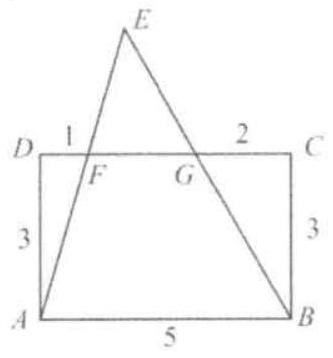
\includegraphics[width=\textwidth]{images/088(2).jpg}

\section*{Solution}
Solution not available.

\end{document}
